\documentclass{article}
\usepackage[utf8]{inputenc}
\usepackage{caption}
\usepackage[margin=1in]{geometry}
\usepackage{graphicx}
\usepackage{pdfpages}
\usepackage{float}
\pdfminorversion=7

\begin{document}
\begin{titlepage}


\centering
\vspace*{2cm}
{\Huge Final Project Document\par}
\vspace{.25cm}
{\LARGE Course Evaluation System\par}
\vspace{1cm}
{\Large Team EVAL\par}
\vspace{.2cm}
{\Large Jovon Craig, Sam Elliott, Robert Judkins, and Stanley Small\par}
\vspace{1cm}
{\Large Client: Dr. Harlan Onsrud\par}
\vspace{1cm}
{\Large December 19, 2018\par}
\vspace{11cm}

University of Maine - Fall of 2018 - COS 397

Instructor: Professor Terry Yoo

\end{titlepage}

\newpage

\begin{center}
{
\includegraphics[scale=.2]{images/team_logo.png}} \\ 	\bigskip
{\LARGE Course Evaluation System } \\ \medskip
{\large Final Project Document } \\ \medskip
\end{center}

\tableofcontents

\newpage

\section{Introduction}
 

\subsection{Purpose of This Document}

This final project document gives an overview of our course evaluation system, the purpose of it, and why we believe it is so useful. We first talk about existing survey creation software and how they are not tailored to college instructors and administrators, unlike our system. The next section goes into more detail about the system, discussing its requirements, user interface, and architecture. The section mentions what we will deliver to the client and our progress on creating the system. The conclusion talks about the steps we still need to take to successfully complete the project.

This document is intended for the development team, the product client, and potential users of the system. Team EVAL needs this document to see whether the evaluation system is implemented in code properly. The client, Professor Harlan Onsrud, also needs it to verify that we are designing the system according to his needs. The document helps the software's users by informing them how the system specifically helps them with their work.

\subsection{References}

Craig, J., Elliott, S., Judkins, R., \& Small, S. 29 October 2018. \textit{System Requirements Specification.}
\vspace{3mm}\newline
Craig, J., Elliott, S., Judkins, R., \& Small, S. 16 November 2018. \textit{System Design Document.}
\vspace{3mm}\newline
Craig, J., Elliott, S., Judkins, R., \& Small, S. 30 November 2018. \textit{User Interface Design Document.}
\vspace{3mm}\newline
Onsrud, H. ``Example Question Selection Form.'' See Appendix D.
\vspace{3mm}\newline
Onsrud, H. ''Report for Professor: Roy Turner'' See Appendix E.
\vspace{3mm}\newline
LimeSurvey: The online survey tool - open source surveys. (n.d.). Retrieved from

https://www.limesurvey.org/.

\section{Purpose of This System}

\subsection{Our Problem}

In 2015, there were more than 4,600 higher-education institutions in the United States. Virtually all of them offer a breadth of college courses for students to complete and take them through their academic careers. At the end of a course, students typically fill out an evaluation survey so that teachers know what they are doing right and wrong. Unfortunately, many institutions, such as the University of Maine, are behind in using technology for this task.

The University of Maine has traditionally used Scantron sheets for course evaluation forms. As Team EVAL knows, filling in tiny bubbles with pencil and paper is tedious. It is also hard work for the college administration to use Scantron sheets. They need to scan the forms for every student in every course, and the data then needs to be collected in a form that is readable for instructors. The University of Maine must upgrade to keep with the times and exploit today's technology.

\subsection{Existing Survey Software}

Several software solutions currently exist that allow users to create, modify, and publish surveys. One notable example is LimeSurvey, a free and open-source tool that is operated online. The team acknowledges the immense amount of work put into creating LimeSurvey, with its selection of question types, scalability, visualization features, and other powerful functionality. However, LimeSurvey has always been general-purpose software; it is aimed at multiple types of users who want to make surveys.

College teachers and administrators need to jump through hoops to use a tool like LimeSurvey. Their surveys are highly standardized and they are sent to potentially hundreds of students. LimeSurvey and similar software do not account for these qualities. A college instructor would have to manually input every field, question, and class roll into each survey from scratch.  UMaine is using another service, Blue by Explorance, that has the necessary functionality, but it is expensive to afford. Those are some of the reasons why our client, Dr. Onsrud, wants us to create an evaluation system better suited to instructors.

\subsection{Our Solution}

Our solution to the above problems is to make our own free and open-source course evaluation system, which has simplicity and ease-of-use in mind. Like existing survey software, our system can too create, modify, and publish surveys. But the differences between our software and LimeSurvey are great. With the new system, instructors and administrators can select a survey created previously to use again for a different survey. They can modify the class roll at the same time as they modify their evaluation form. Also, survey results are specially displayed to indicate the current performance of an instructor.

There are several way in which users can interact with our novel course evaluation system. First, they can create a new evaluation survey form with any required fields and questions already listed. They can then edit forms that are unpublished or view forms that have already been published. After publishing a survey, students are periodically reminded to complete it by our system. Finally, users can see results on a select group of college courses for each question in a survey.

\section{About This System}

\subsection{System Requirements}

\subsection{System Architecture}

\begin{center}
\captionof{figure}{Component diagram of the system}
\vspace{2mm}
\label{fig:componentdiagram}
{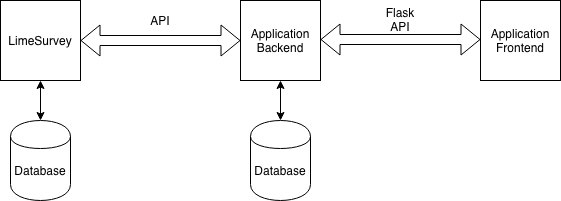
\includegraphics[scale=.75]{images/component_diagram.png}} 
\end{center}

\subsection{User Interface}

\begin{center}
\begin{figure}[H]
    \centering
    \caption{Home screen of the user interface}
    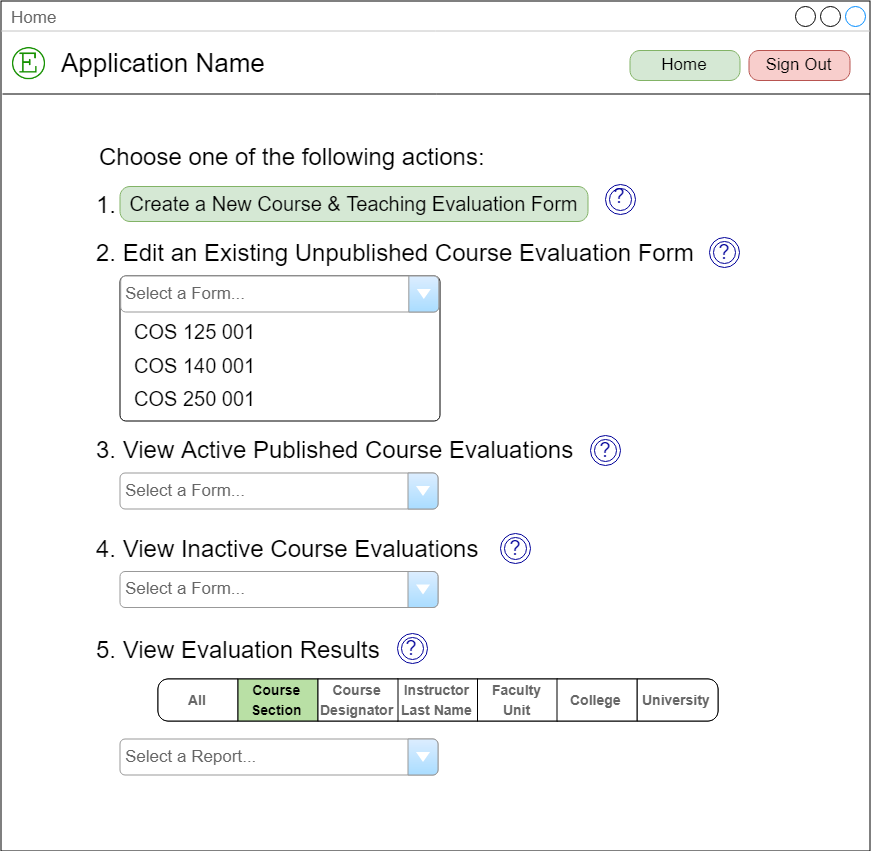
\includegraphics[width=6.5in]{images/home_screen.png}
\end{figure}
\end{center}

\subsection{Tests}

Team EVAL will write several tests in the near future to ensure that the course evaluation system meets all system requirements.

\section{Conclusion}

\subsection{Needs This System Meets}

\subsection{Current Progress}
We have met with our client, Professor Harlan Onsrud, several times over the past few months. Initially we met him to solitic the requirements for the product so that we could deliver something that would both satisfy our customer and potential users of the system. Though it took some time, we eventually came to an agreement, and the requirements were written in detail for us to refer to during development. See the System Requirements Specification for more detail.
	
Next, we started designing our system and the seperate components that would be in our implementation, including the front-end user interface, database, API, and the third-party software LimeSurvey. Each component interacts with each other to combine to our final product. Once again, we sat down with our client to discuss the system architecture and he was eventually satisfied with our design. View Appendix ?? to see the full System Design Document.

Once the requirements and architecture were decided, we had to design the user interface of the product. This is arguably the most important part, as this is what the user would be interacting with when using the product. After conferring with our client, we drew up a simple UI that would be easy for the user to use and understand. See the User Interface Design Document for more detail.

The database that will store all our user's class survey data is in development. The database schema is finished, and we wrote a script to create it and some mock data. An API is also in development that will help us interface our system with the existing LimeSurvey system. The team has most of the API's endpoints finished, but no tests have been written yet. We have also finished a simple prototype that will allow a user to view all screens of the final product. It is not entirely interactive at the moment, but it gives a glimpse of what the final product may become.

\subsection{Next Steps}

There is still a lot of work to do before our evaluation system is complete. First, the team will finish implementing all endpoints in the API. We will also write helper functions that use the LimeSurvey API to publish surveys and retrieve responses. The user interface prototype will be polished to match what our wireframes specify, and the front-end will include functions that interact with the API and the database. Finally, we plan to write a series of tests for the back end and front end to debug the software and know when we are finished with the system.

The team will create an administrator manual and user manual to tell potential users how to interact with the evaluation system. Near the end of the school year, we will submit the final copies of all of our documents electronically. Table ?? lists the date and format that each submission from Team EVAL has been or will be delivered. The dates for incomplete submissions are estimated.

\begin{center}
\captionof{table}{}
\begin{tabular}{|p{6cm}|p{3cm}|p{3cm}|} 
\hline
\textbf{Submission} & \textbf{Date of Delivery} & \textbf{Format} \\
\hline
System Requirements Specification & 10/29/2018 & Hard Copy\\ 
\hline
System Design Document & 11/16/2018 & Hard Copy\\ 
\hline
User Interface Design Document & 11/30/2018 & Hard Copy\\ 
\hline
Administrator Manual & April 2019 & Hard Copy\\ 
\hline
User Manual & May 2019 & Hard Copy\\ 
\hline
System Requirements Specification & May 2019 & Electronic\\ 
\hline
System Design Document & May 2019 & Electronic\\ 
\hline
User Interface Design Document & May 2019 & Electronic\\ 
\hline
Administrator Manual & May 2019 & Electronic\\ 
\hline
User Manual & May 2019 & Electronic\\ 
\hline
Source Code & May 2019 & Electronic\\ 
\hline
Web Link to Program & May 2019 & Electronic\\ 
\hline
\end{tabular}
\end{center}


\newpage
\section{Agreement Between Customer and Contractor}
This page shows that all members of Team EVAL and the client, Harlan Onsrud, have agreed on all the information in the final project document. By signing this document, Team EVAL and Dr. Onsrud approve of everything stated about the course evaluation system.

The team will follow a process in the case that the final document is changed after we sign it. First, the team will write a rough draft of the changes to be made to the document. Second, all team members and Harlan Onsrud will sign the document agreeing to the changes. Finally, the team will make the changes to the final copy of the document.

\vspace{.7in}
\noindent
\begin{tabular}{ p{5cm} p{5cm} p{5cm} } 
\textbf{\textit{Name}} & \textbf{\textit{Signature}} & \textbf{\textit{Date}} \\[.5cm]
\textbf{Jovon Craig} & $\rule{5cm}{.1mm}$ & $\rule{5cm}{.1mm}$\\[.5cm]
\textbf{Sam Elliott} & $\rule{5cm}{.1mm}$ & $\rule{5cm}{.1mm}$\\[.5cm]
\textbf{Robert Judkins} & $\rule{5cm}{.1mm}$ & $\rule{5cm}{.1mm}$\\[.5cm]
\textbf{Stanley Small} & $\rule{5cm}{.1mm}$ & $\rule{5cm}{.1mm}$\\[.5cm]
\textbf{Harlan Onsrud} & $\rule{5cm}{.1mm}$ & $\rule{5cm}{.1mm}$\\[.5cm]
Customer Comments: & \multicolumn{2}{ l }{ $\rule{10.45cm}{.1mm}$ }\\[.5cm]
\multicolumn{3}{ l }{ $\rule{15.9cm}{.1mm}$ }\\[.5cm]
\end{tabular}

\newpage
\section{Team Review Sign-off}

This page shows that all members of Team EVAL have reviewed the final project document and agreed on its content. By signing this document, the team members agree that all information about the evaluation system's purpose, requirements, user interface, and architecture, as well as the work the team plans to do in the future.

\vspace{.7in}
\noindent
\begin{tabular}{ p{5cm} p{5cm} p{5cm} } 
\textbf{\textit{Name}} & \textbf{\textit{Signature}} & \textbf{\textit{Date}} \\[.5cm]
\textbf{Jovon Craig} & $\rule{5cm}{.1mm}$ & $\rule{5cm}{.1mm}$\\[.5cm]
Comments: & \multicolumn{2}{ l }{ $\rule{10.45cm}{.1mm}$ }\\[.5cm]
\multicolumn{3}{ l }{ $\rule{15.9cm}{.1mm}$ }\\[.5cm]
\textbf{Sam Elliott} & $\rule{5cm}{.1mm}$ & $\rule{5cm}{.1mm}$\\[.5cm]
Comments: & \multicolumn{2}{ l }{ $\rule{10.45cm}{.1mm}$ }\\[.5cm]
\multicolumn{3}{ l }{ $\rule{15.9cm}{.1mm}$ }\\[.5cm]
\textbf{Robert Judkins} & $\rule{5cm}{.1mm}$ & $\rule{5cm}{.1mm}$\\[.5cm]
Comments: & \multicolumn{2}{ l }{ $\rule{10.45cm}{.1mm}$ }\\[.5cm]
\multicolumn{3}{ l }{ $\rule{15.9cm}{.1mm}$ }\\[.5cm]
\textbf{Stanley Small} & $\rule{5cm}{.1mm}$ & $\rule{5cm}{.1mm}$\\[.5cm]
Comments: & \multicolumn{2}{ l }{ $\rule{10.45cm}{.1mm}$ }\\[.5cm]
\multicolumn{3}{ l }{ $\rule{15.9cm}{.1mm}$ }\\[.5cm]
\end{tabular}


\newpage
\section{Document Contributions}

Stanley Small ??. Stan contributed about ?? percent of the document.

Jovon Craig ??. Jovon contributed about ?? percent of the document.

Sam Elliott ??. Sam contributed about ?? percent of the document.

Robert Judkins ??. Robert contributed about ?? percent of the document.

\newpage

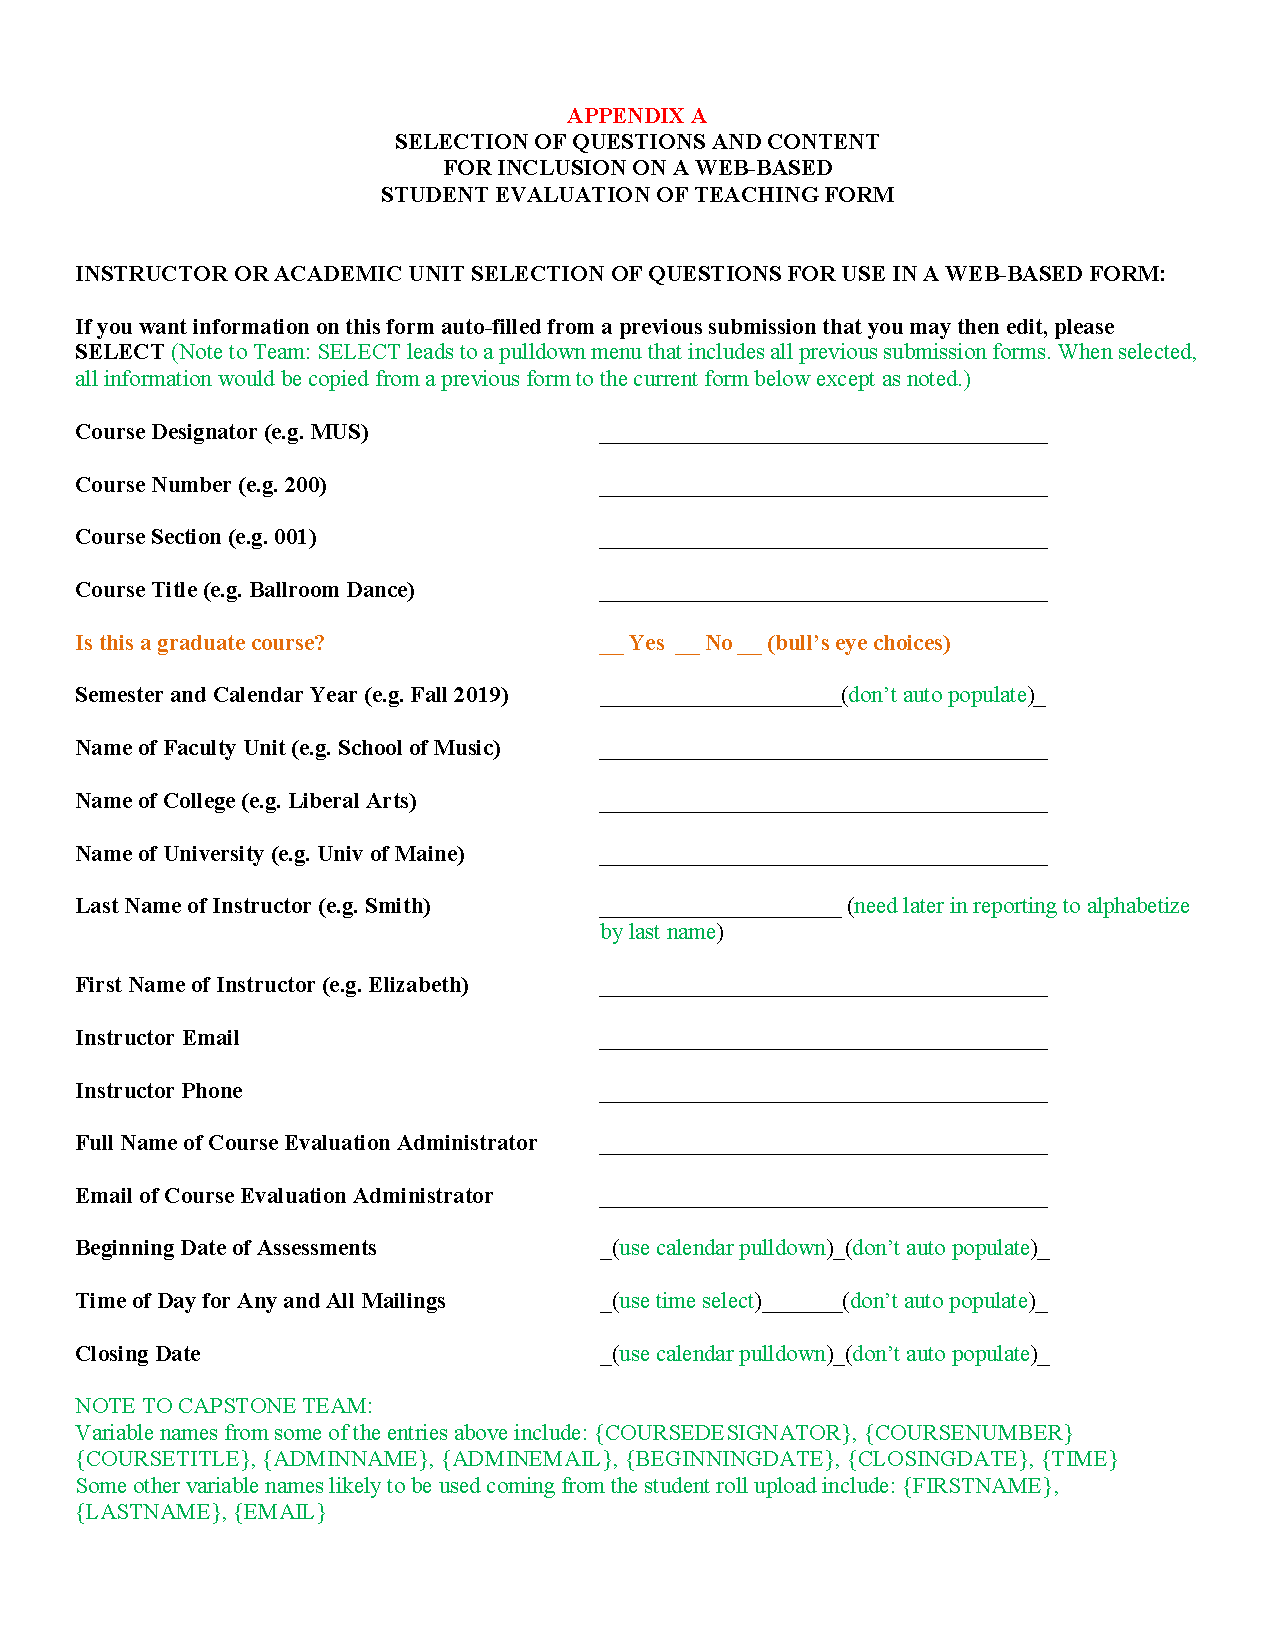
\includepdf[scale=0.85,pages=1,pagecommand=\section{Example Question Selection Form}]{images/question_appendix.pdf}
\includepdf[scale=0.85,pages=2-]{images/question_appendix.pdf}

\newpage

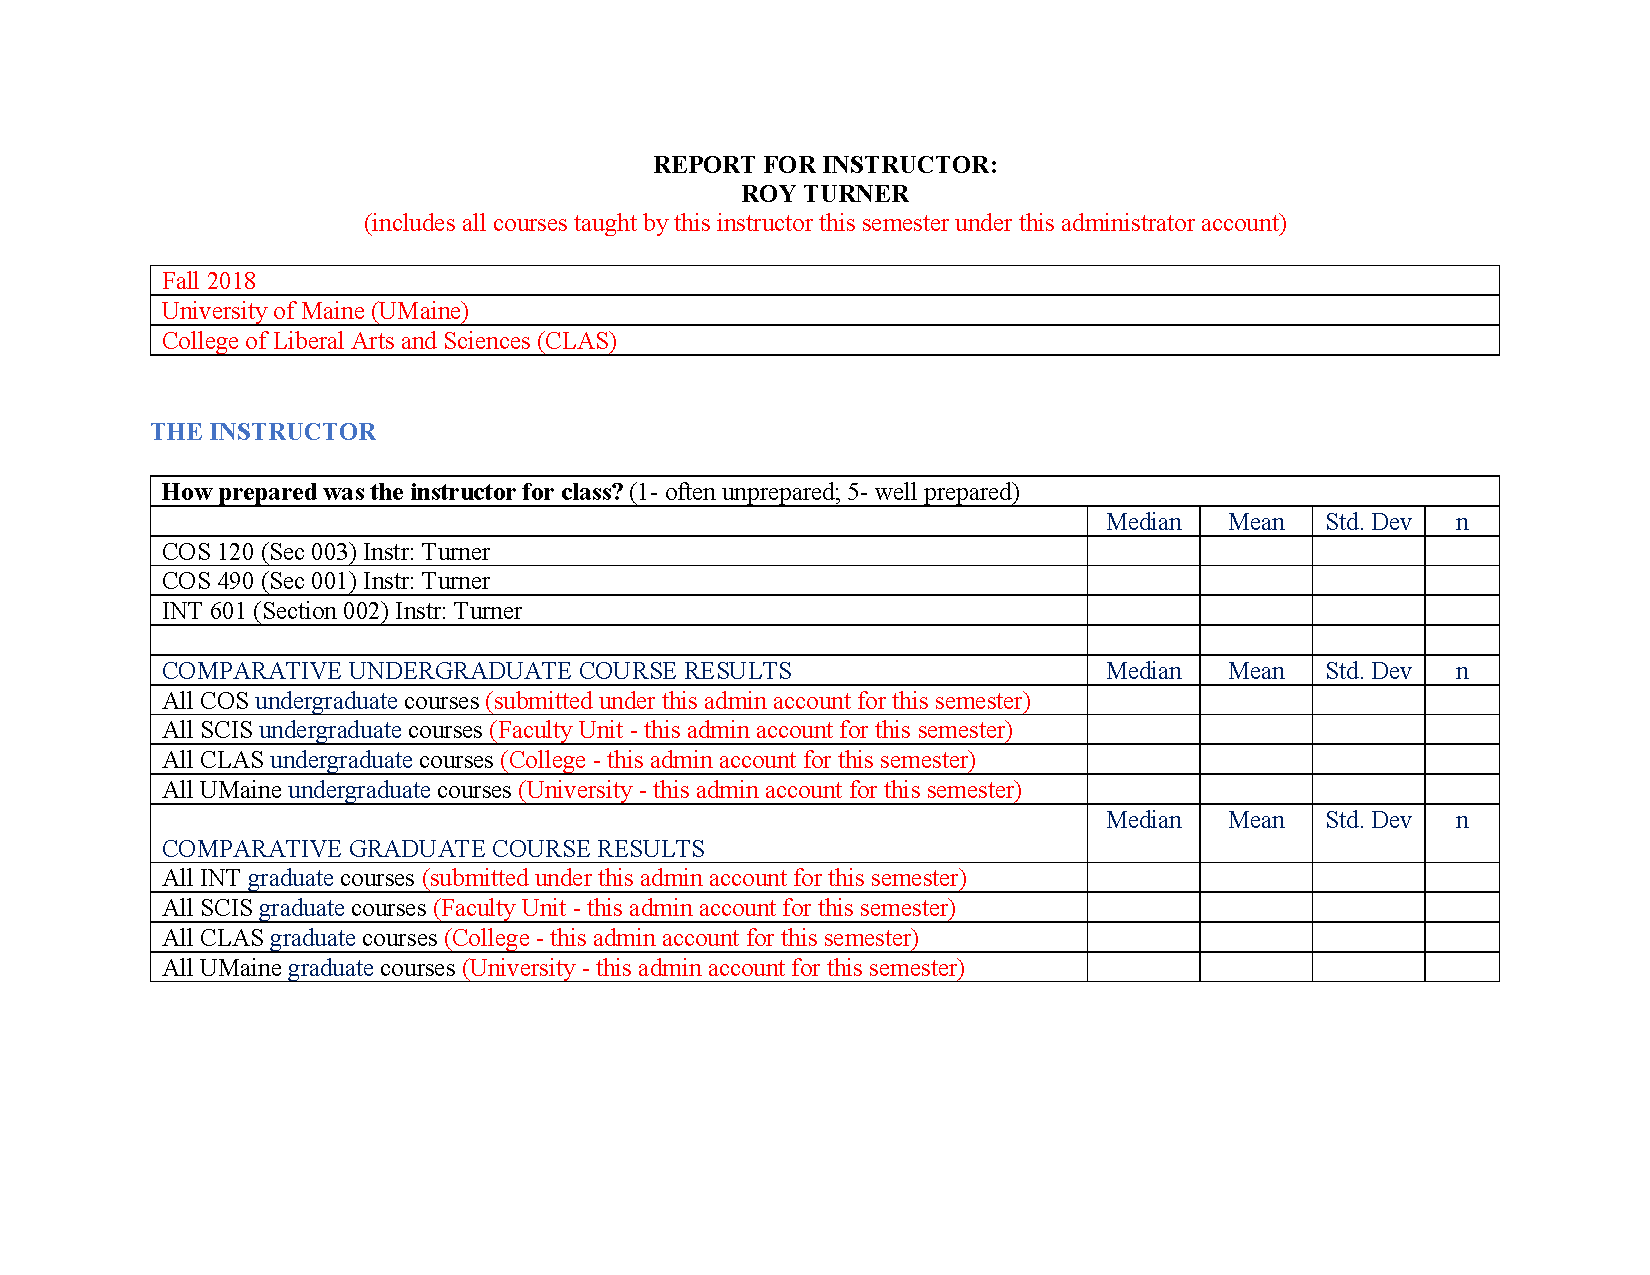
\includepdf[scale=0.92,pages=1,pagecommand=\section{Example Results Display}]{images/results_appendix.pdf}
\includepdf[scale=0.92,pages=2-]{images/results_appendix.pdf}
\end{document}
